\documentclass{standalone}
\usepackage{pgfplots}
\begin{document}
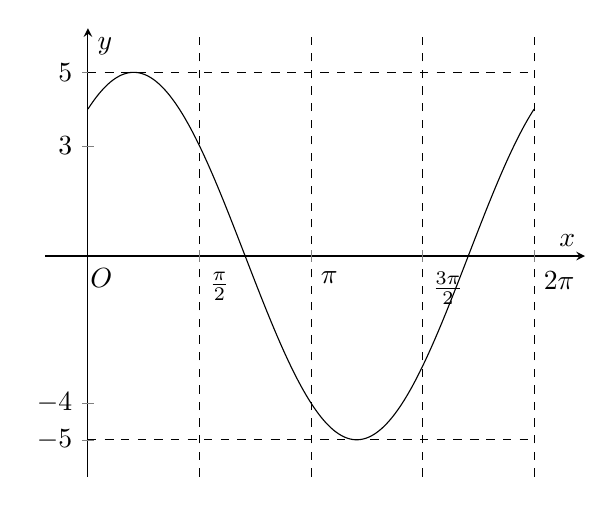
\begin{tikzpicture}
\begin{axis}
[
ymin=-6,ymax=6.2,
xmin=-0.6,xmax=7,
xtick=\empty,
ytick=\empty,
extra x ticks={1.5708, 3.14159, 4.71239, 6.28319},
extra x tick labels={$\frac{\pi}{2}$, $\pi$, $\frac{3\pi}{2}$, $2\pi$},
extra y ticks={-5, -4, 3, 5},
extra y tick labels={$-5$, $-4$, $3$, $5$},
every extra x tick/.style={
    xticklabel style={anchor=north west},
    grid=major,
    major grid style={very thin,dashed,black}
},
axis lines = center,
xlabel=$x$,ylabel=$y$,
samples=200,
]
\addplot [black, domain=0:6.28319] {3*sin(deg(x)) + 4*cos(deg(x))};
\addplot [black, dashed, domain=0:6.28319] {5};
\addplot [black, dashed, domain=0:6.28319] {-5};
\node at (axis cs:0.19, -0.61) {$O$} ;
\end{axis}
\end{tikzpicture}
\end{document}
